\section{Classics}
\label{s:classics}
Various works that do not entirely rely on learning algorithms, be them deep or statistical, are reviewed.
The majority of these come from the pre deep learning era.
The discussion of this section is not strictly about the papers, but about the methodology of the time.

%%%%%%%%%%%%%%%%%%%%%%%%%%%%%%%%%%%%%%%%%
%              Hoeim
%%%%%%%%%%%%%%%%%%%%%%%%%%%%%%%%%%%%%%%%%
\subsection{Hoeim et al.}
Derek Hoeim and his collaborators produced a sequence of works on "scene interpretation" \cite{autopopup1, autopopup2, autopopup3, autopopup4, autopopup5, autopopup6}.
Only the first will be discussed in detail.

% architecture
\begin{figure}
	\centering
	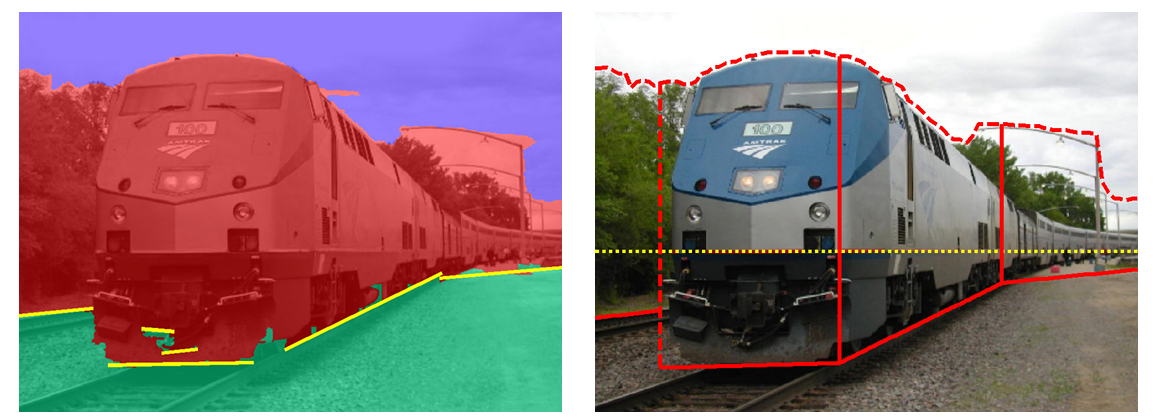
\includegraphics[scale=0.3]{figs/hoeim}
	\caption{Hoeim et al. method \cite{autopopup1}. Left: segmentation and lines fitting; Right: building the 3D model. \label{fig:hoeim}}
\end{figure}

In \cite{autopopup1} the objective is to do a simple reconstruction of the scene geometry by building a 3D model.
The reconstruction procedure is based on strong assumptions that are: the scene is composed by a ground, vertical objects stick to it and an infinite distant sky.
This obviously only work for outdoor scenes.
The ground is modeled as a plane and vertical objects as little segments of planes perpendicular to the ground and parallel to the image plane.
The pipeline is based on three phases:
\begin{enumerate}
	\item{Segmenting the image into "ground", "vertical" and "sky"}
	\item{Cleaning the segmentation}
	\item{Fitting lines to the segmented vertical regions and building the 3D model}
\end{enumerate}
In figure \ref{fig:hoeim} there is an example.
Another major assumptions is the absence of occlusion between objects.
If occlusion occurs, the segmentation procedure is not able to distinguish between different object by other means that some ground pixels in between.
Hence, in the case of occlusion, two objects at completely different depths would result in the closest to the camera.

Hoeim et al. deal with occlusion in \cite{autopopup4}, where they try to model the occlusion cues and build a computational method for occlusion detection.
The method uses a Conditional Random Field (CRF).
It was a very used statistical method in computer vision before deep learning, its main drawback is the expensive inference that involves a global optimization step.
In last years neural CRFs have been proposed also for single image depth estimation, although I will not review them.

In \cite{autopopup2} and \cite{autopopup5} the problem of the surface orientation prediction is tackled.
The idea, also found in older works like \cite{VideoCompass}, was to group surface normals into a predefined way.
For instance: pointing upward, pointing downward, pointing left or pointing right.
The result was a segmentation method.
At this time, for segmenting images, the main approach was to first do an over segmentation by dividing the image into super-pixels.
A super-pixels are groups of pixels that share some local property.
Second, associate to each super-pixel various numerical features, such as the histogram of colors, the number of pixels, the mean magnitude of the gradient, ...
These features were hand-crafted, in the sense that they are not learned and someone explicitly thought about them and tested them in some scenarios.
Doing so, each super-pixel has numbers associated to it.
Using a dataset of segmented images one could train a statistical learning method (e.g. a boosting method or a simple linear regression) to predict the correct labels for a given superpixel.
If the super-pixel information was not sufficient due to its locality, global optimization methods like Random Fields could have been used or iterative grouping (e.g. producing constellations of super-pixels by grouping them) was performed.

Continuing the journey of Hoeim et al., in \cite{autopopup3} the focus is on the objects.
In here object detection is tackled and the authors also attempt to orient detected objects in space.

All of these works lead to "Closing the Loop in Scene Interpretation" \cite{autopopup6} were they are all put together in a complex pipeline for building a 3D model of the scene as rich as possible.